%%%%%%%%%%%%%%%%%%%%%%%%%%%%%%%%%%%%%%%%%%%%%%%%%%%%%%%%%%%%%%%%%%%%%%%%%%%%%%%
\section{Aula 02}
%%%%%%%%%%%%%%%%%%%%%%%%%%%%%%%%%%%%%%%%%%%%%%%%%%%%%%%%%%%%%%%%%%%%%%%%%%%%%%%

%%%%%%%%%%%%%%%%%%%%%%%%%%%%%%%%%%%%%%%%%%%%%%%%%%%%%%%%%%%%%%%%%%%%%%%%%%%%%%%
\subsection{Definição de algoritmo}

\begin{itemize}
\item Procedimento bem definido que:
	\begin{itemize}
	\item recebe como entrada um valor, ou conjunto de valores
	\item produz como saída um valor ou conjunto de valores
	\end{itemize}
\item Conjunto de passos que transforma a entrada na saída.
\item Exemplo do {\bf problema de ordenação}:
\end{itemize}

{\bf Entrada}: uma sequência de $n$ números $\langle a_1, a_2, ..., a_n \rangle$.

{\bf Saída}:  Uma permutação $\langle {a'}_1, {a'}_2, ..., {a'}_n \rangle$ da
entrada tal que ${a'}_1 \leq {a'}_2 \leq ... \leq {a'}_n \rangle$.

\begin{itemize}
\item Essa entrada do algoritmo é uma {\bf instância} do problema.
\item Para um algoritmo estar {\bf correto}, para cada instância, ele termina com saída 
correta. Um algoritmo correto \textsf{resolve} um problema. 
\end{itemize}

Exemplos de problemas:
\begin{itemize}
\item O Projeto do Genoma Humano para identificar todos os genes do DNA humano.
\item Internet com descoberta de rotas.
\item E-commerce.
\end{itemize}

%%%%%%%%%%%%%%%%%%%%%%%%%%%%%%%%%%%%%%%%%%%%%%%%%%%%%%%%%%%%%%%%%%%%%%%%%%%%%%%
\subsection{Análise de algoritmos}

\begin{itemize}
\item Medida de custo de execução de um programa.
\item Importante separar entre uma medida {\bf real}  e {\bf generalizada}.
	\begin{itemize}
	\item real depende do compilador, hardware, memória, etc.
	\item generalizada pode usar um computador abstrato para análise.
		\begin{itemize}
		\item Ex: máquina teóricas (Turing, lambda).
		\end{itemize}
	\end{itemize}
\item Grande parte dos casos utiliza-se o número de {\bf elementos de entrada}, denotado $n$, para
determinar o tempo de um algoritmo.
\item Se fosse um grafo, poderia-se usar como $n$ o número de vértices.
\item O {\bf tempo de execução} é o número de passos executados, sendo o mais independente de 
máquina possível.
\end{itemize}

Vamos considerar dois exemplos de algoritmos de ordenação com $n$ elementos de entrada:
\begin{itemize}
\item {\bf Ordenação por inserção} com custo $c_1 n^2$ sendo $c_1$ uma constante que não depende de $n$.
\item {\bf Ordenação merge sort} com custo $c_2 n \log n$ sendo $c_2$ outra constante que não depende de $n$.
\end{itemize}

Considere um exemplo onde vamos executar a ordenação por inserção em uma máquina mais rápida (A)
e a ordenação por mergesort em uma máquina mais lenta (B).
A entrada será de 10 milhões de números ($10^7$ ou equivalente a $80$ MB).
Suponha que a máquina A executa $10^10$ instruções por segundo, enquanto que a máquina B executa
somente $10^7$ instruções por segundo. 
Ainda, o código da inserção tem custo $2n^2$ enquanto que o mergesort tem $50n \log n$ de custo.

Para ordenar $10^7$ números, o computador A com ordenação por inserção demora
\begin{equation*}
\frac{2\dot (10^7)\; instrucoes}{10^{10}\; instrucoes/segundo} = 20.000 \; segundos.
\end{equation*}

Depois, para ordenar os $10^7$ números no computador B com mergesort custa
\begin{equation*}
\frac{50 \dot (10^7)\; instrucoes}{10^{7}\; instrucoes/segundo} = 1.163 \; segundos \;(20\; minutos).
\end{equation*}

%%%%%%%%%%%%%%%%%%%%%%%%%%%%%%%%%%%%%%%%%%%%%%%%%%%%%%%%%%%%%%%%%%%%%%%%%%%%%%%
\subsubsection{Função de complexidade}

O custo de um algoritmo é definido em geral por uma função de complexidade $f$. Sendo assim,
$f(n)$ é a medida de tempo de execução de um algoritmo para uma instância do problema de tamanho $n$.
Podemos ter uma função $f(n)$ que descreve:
\begin{itemize}
\item Complexidade de {\bf tempo} onde $f(n)$ mede o tempo para executar um problema $n$.
\item Complexidade de {\bf espaço} onde $f(n)$ mede o espaço de memória ocupado pelo algoritmo
com entrada $n$.
\end{itemize}

Caso nada for mencionado, estamos falando sobre complexidade de tempo em grande parte do material.

%%%%%%%%%%%%%%%%%%%%%%%%%%%%%%%%%%%%%%%%%%%%%%%%%%%%%%%%%%%%%%%%%%%%%%%%%%%%%%%
\subsubsection{Analise simples - maior elemento}

\begin{figure}[!htb]
\centering
\begin{framed}
\begin{lstlisting}
int Max( int *A, int n ){
	int i, temp;
	temp = A[0];
	for( i = 1; i < n; i++ ){
		if( temp < A[i] )
			temp = A[i];
	}
	return temp;
}
\end{lstlisting}
\end{framed}
\caption{Algoritmo que encontra o maior elemento.}
\end{figure}

Seja $f(n)$ a função de complexidade que determina o número de comparações entre elementos de $A$.
Logo, $f(n) = n - 1$, para $n > 0$.

No caso do algoritmo de maior elemento, o custo de execução é uniforme sobre todos os problemas 
de tamanho $n$.

%%%%%%%%%%%%%%%%%%%%%%%%%%%%%%%%%%%%%%%%%%%%%%%%%%%%%%%%%%%%%%%%%%%%%%%%%%%%%%%
\subsubsection{Analise da ordenação por inserção}

O código da figura~\ref{aula02:algo:insertion} mostra o algoritmo da ordenação
por inserção, enquanto a figura~\ref{aula02:fig:insertion} apresenta os passos
na ordenação de 6 números.
%
\begin{figure}[!htb]
\centering
\begin{framed}
\begin{lstlisting}
void Insercao( int *A, int n ) {
	int i, j;
	int x;
	for( j = 2; j <= n; j++ ){
		x = A[j];
		i = j - 1;
		while( i > 0 && x  < A[i] ){
			A[i+1] = A[i];
			i--;
		}
		A[i+1] = x;
	}
}
\end{lstlisting}
\end{framed}
\caption{Algoritmo de ordenação por inserção.}
\label{aula02:algo:insertion}
\end{figure}
%
\begin{figure}[ht]
\centering
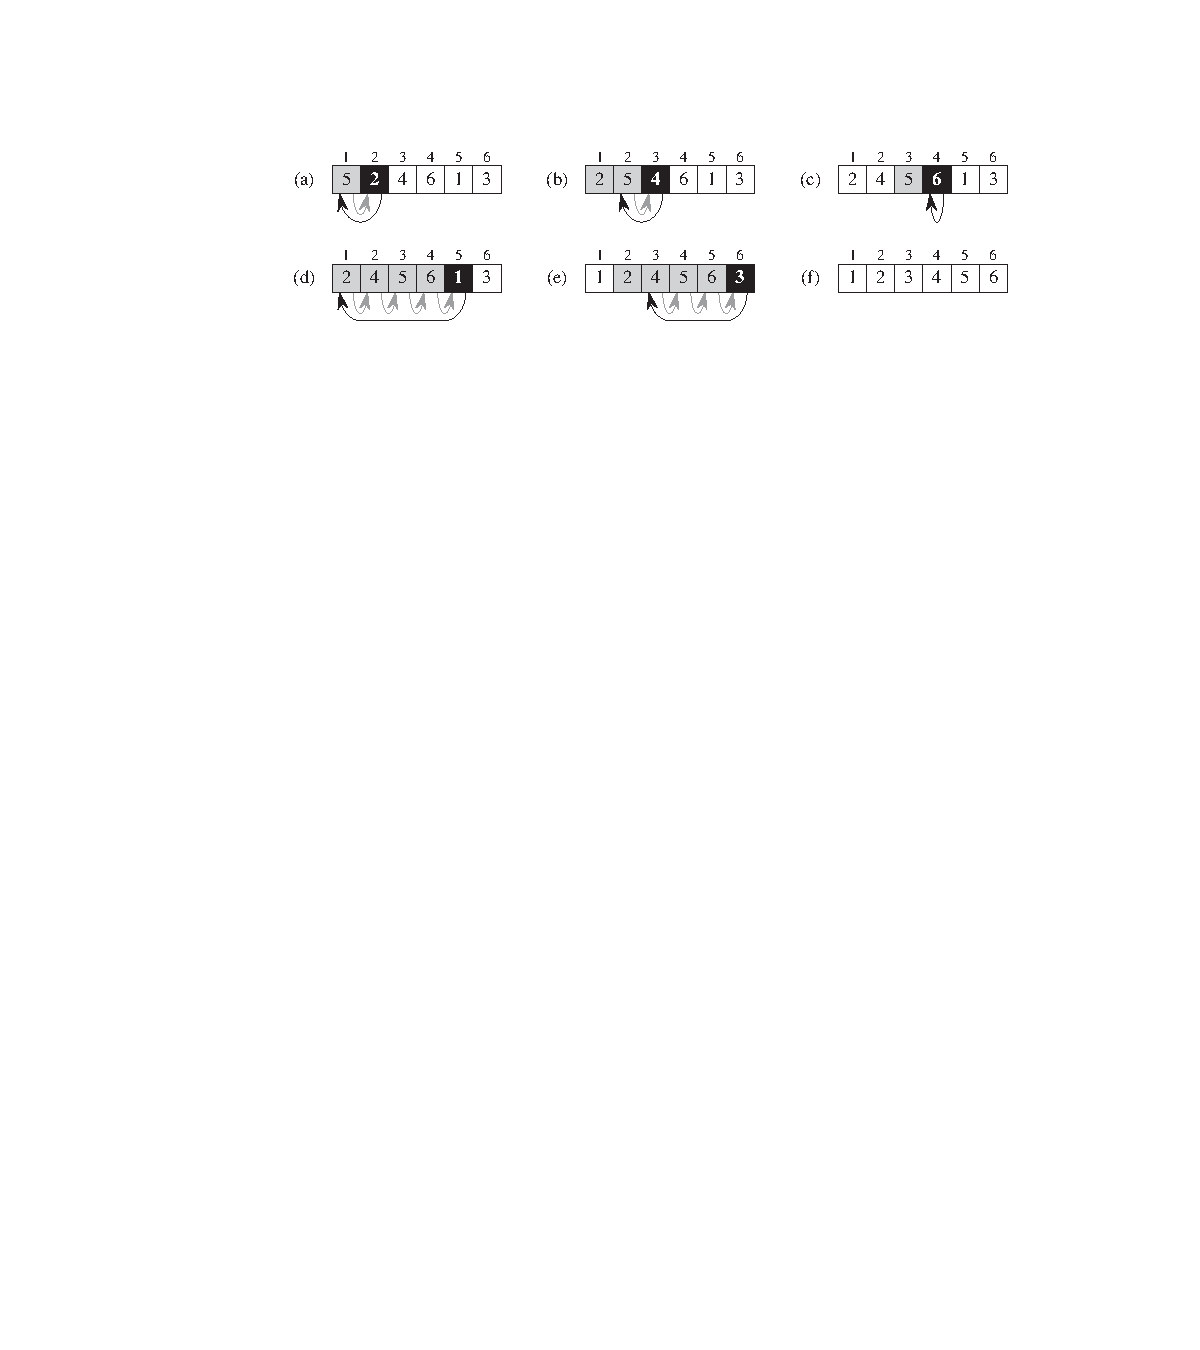
\includegraphics[width=0.8\textwidth]{02-insertionsort}
\caption{Passos da ordenação por inserção.}
\label{aula02:fig:insertion}
\end{figure}

A ordem dos elementos na ordenação por inserção depende do tamanho da entrada $n$. 
Além disso, o tempo de execução pode variar conforme a ordem dos elementos.
%
O tempo de execução depende da soma dos tempos de execução de cada passo do algoritmo
executado: se o passo tem custo $c_i$ e executa $n$ vezes contribui $c_i n$ para o tempo
total.
Assumind o pior caso, quando a entrada está em ordem reversa, o custo de execução é 
$an^2 + bn +c$ para constantes $a$, $b$ e $c$.


%%%%%%%%%%%%%%%%%%%%%%%%%%%%%%%%%%%%%%%%%%%%%%%%%%%%%%%%%%%%%%%%%%%%%%%%%%%%%%%
\subsubsection{Melhor caso, caso médio e pior caso}

Em alguns algoritmos, o custo de execução também é uma função da entrada de dados, não somente
do tamanho $n$ da entrada.
No exemplo anterior, demostramos apenas o pior caso. 
Os possíveis casos para análise são:
\begin{itemize}
\item Pior caso quando os elementos estão em ordem inversa e todos os elementos 
são trocados.
Sabendo o pior caso, o custo do algoritmo nunca é maior que $f(n)$.
O custo seria $an^2 + bn +c$ para constantes $a$, $b$ e $c$.

\item Melhor caso onde os elementos já estão ordenados e nenhuma troca é necessária.
O custo é $an + b$ para constantes $a$ e $b$.

\item Caso médio pode ser tanto quanto o pior caso. Supondo que aplicamos 
a ordenação por inserção para elementos em ordem aleatória $n$. 
O resultado de uma execução de caso médio será quadratica ($an^2 + bn +c$)
tal como o pior caso.
\end{itemize}


%%%%%%%%%%%%%%%%%%%%%%%%%%%%%%%%%%%%%%%%%%%%%%%%%%%%%%%%%%%%%%%%%%%%%%%%%%%%%%%
\subsubsection{Ordem de crescimento}

A {\bf ordem de crescimento} é uma forma de simplificar a analise de algoritmos.
Nesse caso, consideramos apenas os termos maiores (como $an^2$) sendo que
valores grandes de $n$ são termos relativamente insignificantes.

Na tabela abaixo, é possível comparar as diferentes funções de crescimento e 
o tempo de execução de acordo com a entrada.
\begin{table}[ht]
\centering
\begin{tabular}{cccccc}
\hline
{\bf descrição} & {\bf função} & {\bf 2x} & {\bf 10x} & {\bf tempo$10n$} & {\bf tempo $10n$ ($10\times$ rápido)} \\ 
\hline
constante        & $1$ & & & &  \\
linear           & $n$        & $2$ & $10$ & um dia & algumas horas \\
linear-logaritmo & $n \log n$ & $2$ & $10$ & um dia & algumas horas \\
quadratico       & $n^2$      & $4$  & $100$ & algumas semanas & um dia  \\
cúbico           & $n^3$ & $8$ & $1.000$ & meses & algumas semanas  \\
exponencial      & $2^n$  & $2^n$ & $2^{9n}$ & nunca & nunca  \\
\hline
\end{tabular}
\end{table}

%%%%%%%%%%%%%%%%%%%%%%%%%%%%%%%%%%%%%%%%%%%%%%%%%%%%%%%%%%%%%%%%%%%%%%%%%%%%%%%
\subsubsection{Notação assintótica}

A notação assintótica é uma forma de denotar o crescimento de uma função,
e uma notação para comparar algoritmos.
%
\begin{figure}[ht]
\centering
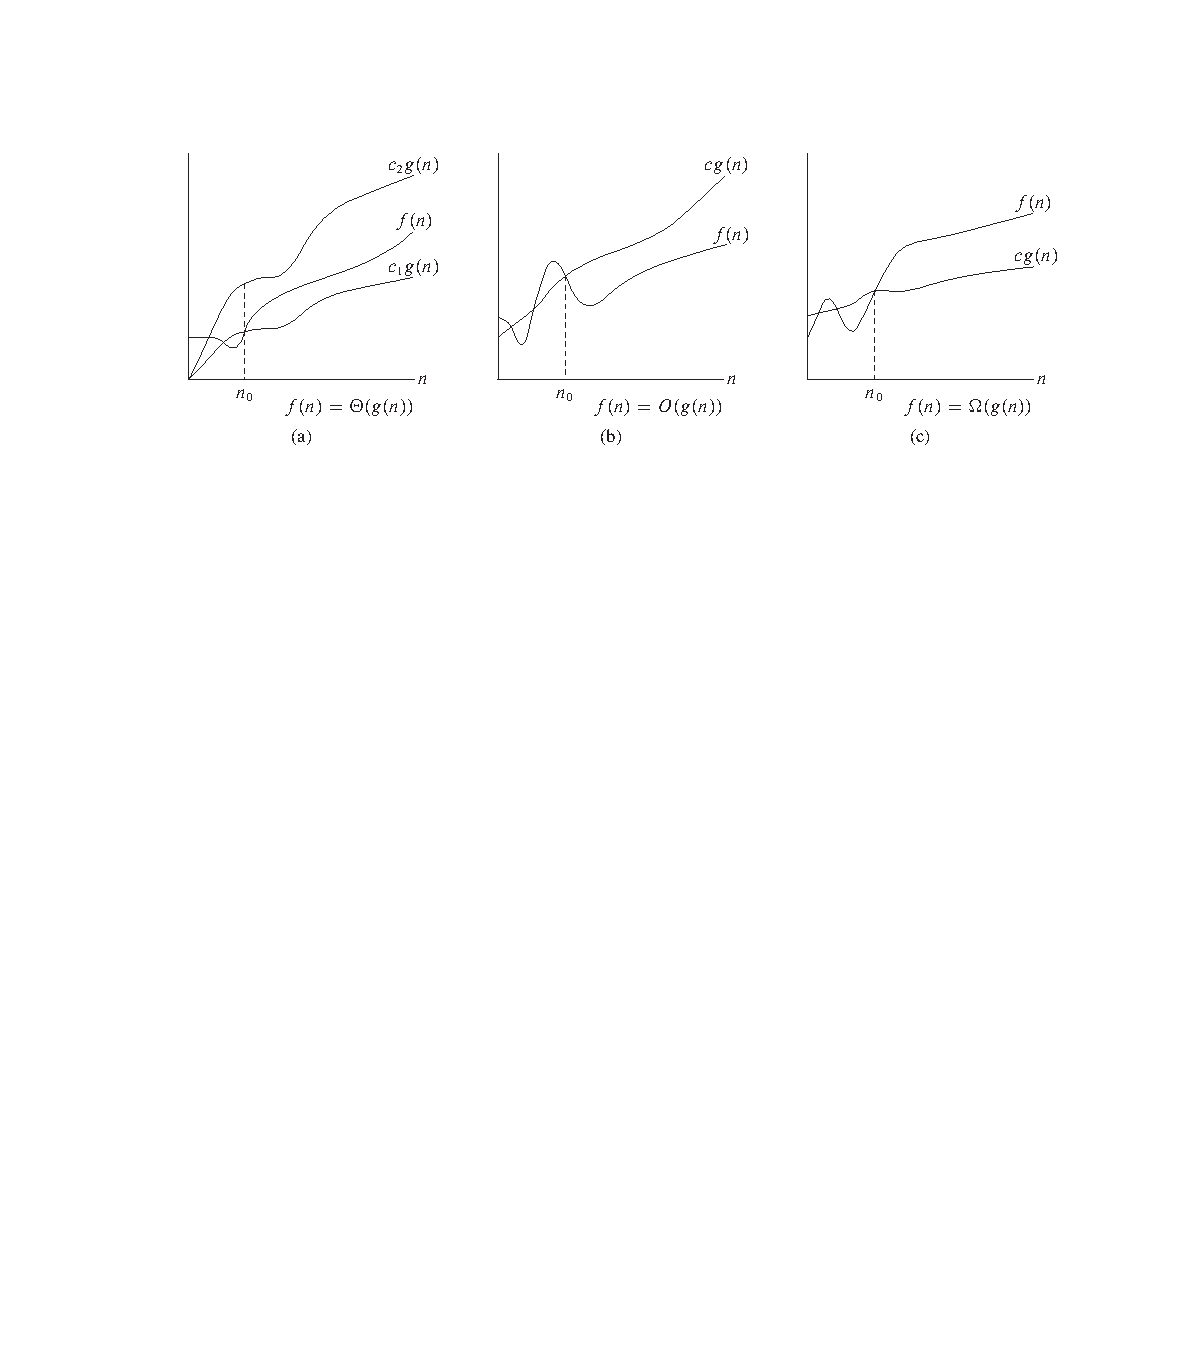
\includegraphics[width=0.8\textwidth]{02-assintotico}
\caption{Comparação das notações $\Theta$, $O$ e $\Omega$.}
\label{aula02:fig:assintotico}
\end{figure}

\begin{itemize}
\item $O$ (\emph{big-oh}) define o {\bf limite assintótico superior}, ou seja, 
limite para o tempo de execução para o pior caso. Escrevemos $g(n) = O(f(n))$ para
expressar que $f(n)$ domina assintoticamente $g(n)$. Para
uma função $g(n)$ define-se $O(g(n))$ o conjunto de funções 
$O(g(n)) = \{f(n):$ existe constantes positivas $c$ e $n_0$ tal que $0 \leq f(n) \leq c g(n)$ 
para todo $n \geq n_0\}$.

\item $\Theta$ é um {\bf limite assintótico firme} onde 
para uma função $g(n)$ define-se $\Theta(g(n))$ o conjunto de funções 
$\Theta(g(n)) = \{f(n):$ existe constantes positivas $c_1$, $c_2$ e $n_0$ tal que 
$0 \leq c_1 g(n) \leq f(n) \leq c_2 g(n)$ 
para todo $n \geq n_0\}$.

\item $\Omega$ é um {\bf limite inferior} onde para uma função $g(n)$ 
define-se $\Omega(g(n))$ o cojunto de funções
$O(g(n)) = \{f(n):$ existe constantes positivas $c$ e $n_0$ tal que $0 \leq c g(n) \leq f(n)$ 
para todo $n \geq n_0\}$.

\end{itemize}

No caso da ordenação por inserção, podemos afirmar que o tempo de execução fica entre
$\Omega(n)$ (melhor caso) e $O(n^2)$ (pior caso).

%%%%%%%%%%%%%%%%%%%%%%%%%%%%%%%%%%%%%%%%%%%%%%%%%%%%%%%%%%%%%%%%%%%%%%%%%%%%%%%
\subsubsection{Eficiência}

\begin{framed}
\centering
Um algoritmo é eficiente quando seu tempo de execução é polinomial.
\end{framed}

